\chapter{Introduction}\label{chap:intro}

\section{Problem Description} 

The cids product suite is a platform for ``building information systems with a special focus on interactive geo-spatial systems'' \autocite[]{cismet-cids-readMe} that need to operate on a combination of heterogeneous and distributed data sets.
 It ``[..] consists of a set of services, applications, software components, management tools, development tools, and application programming interfaces (APIs)[...]'' \autocite[]{cismet-cids-readMe} that already provide ``[...] a considerable number of functionalities required for complex geospatial information systems'' \autocite[]{cismet-cids-readMe} such as user management, access control, search and discovery and data visualisation.
 Figure \ref{fig:cids_building_blocks} depicts the important building blocks of the cids platform.


\begin{figure}
	\centering 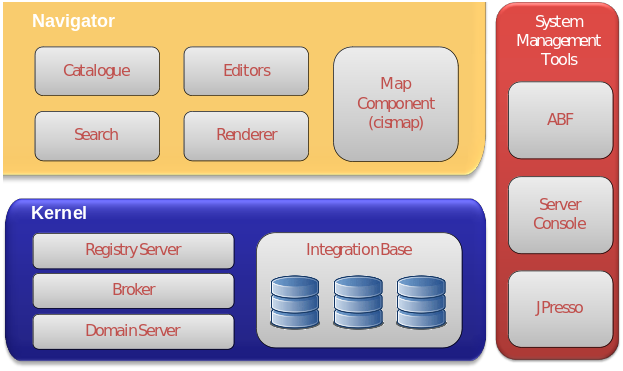
\includegraphics[width=0.8\textwidth]{./img/intro/cids_building_blocks.png}
	\caption{cids building blocks \autocite[]{cismet-cids-readMe}}
	\label{fig:cids_building_blocks}
\end{figure}

Cids is implemented as a distributed system with a client server architecture.
The server components (see blue box in Figure \ref{fig:cids_building_blocks}) are able  to integrate and describe arbitrary objects from many heterogeneous data sources and offer those data in a standardized format to the clients.
Furthermore, the server components are responsible for managing users, user-groups, permissions and many other properties as well as search and discovery of information.

%Hence the different server side components are distributed and decoupled, scalability and reliability are ensured.
 
The yellow building block in Figure \ref{fig:cids_building_blocks} represents the client side of the cids platform, the cids Navigator and its main components.
It is the default client for user interactions with the system.
Among other things, the cids Navigator conjuncts information of the distributed server network and provides it to the user in a user-specific tree view the so called catalogue.
For every object in the catalogue exists a so called renderer and editor.
They provide a graphical user interface for the visualisation of object related information in a user friendly way and allow the user to edit these information.


Just for the sake of completeness, the last building block consists of a set of management tools, that ``support system managers during the installation and maintenance'' \autocite[]{cismet-cids-readMe} of cids based systems but are less important for the following considerations.

Up to now, the cids product suite, which is totally Java based, is not able to offer its services and features to other applications.
Especially the lack of building web applications that uses cids server functionality is a more and more growing issue regarding the incessantly importance of the internet and its more widespread and pervasive usage nowadays.
Therefore one of the latest innovations in the cids platform is a RESTful server API, that offers server side cids functionality to applications in a platform independent way.
This is a immense advancement of the cids platform, hence it creates completely new possibilities in the design of cids based systems and totally new fields of application.


As already mentioned one of the most growing issues is to supplement cids systems with web applications for visualising and editing subsets of the managed data, hence web applications are much more lightweight and thus, easier accessible.
The following example demonstrates this impressively.
A mobile web application can be used for capturing relevant data on site.
Those data could be post-processed with the already existing cids Navigator in a second step.
The rehashed data (or just an interesting subset of it) can then be accessed with the same or an additional web application.
Regarding this example in more detail, it is obvious that such web applications have the same purpose as the already existing Swing based object renderer.


The similar functionality of such html applications and Swing based renderer and editors in the navigator offer the chance to use those web applications as a replacement for the Swing based editors.
This has the benefit of omitting development costs for additional Swing components if an web application with the same purpose is needed anyway.
Thinking one step ahead, it is also imaginable that renderer and editors are solely realized as html applications hence this offers the advantage of a much easier and more spreaded accessibility.Furthermore, the very narrow functionality of the cids RESTful server API, due to its very early stage of development, interferes initial efforts in web application development.
Those efforts are very important and vital at this early phase, hence the cismet company has only slight knowledge in that field of application.

 
% ToDo: make this nice and filthy
Besides these more general and strategic arguments, there is also a specific requirement in one of the EU projects, the cismet company is involved.
Within the CRISMA project many html widgets are implemented that shall simplify the development of decision support systems for Crisis management.
A seamless integration of those html widgets in the cids Navigator is needed.


\section{Objectives}\label{chap:intro-objectives}

Up to now the cids navigator is not able to visualise html applications as object renderer and object editors.
This feature is inevitable for the above mentioned reasons.
Thus, the cids navigator needs to be extended with the respective functionality.
One objective of the presented work is the conceptual design and technical realisation of this feature.
Without going into great detail, it is obvious that this task requires a software component, that is able to parse and visualise html documents similar to existing web browsers.
Furthermore, it is necessary to develop a simple web application that can act as a renderer / editor for a cids objects which simplifies testing and can act as a demo application.
The development of such an first web application is the second objective of this work.

Although it is conceivable (and with the outlined feature quite possible) to use and visualise arbitrary and already existing web applications as renderer and editor components it is not clear if the integration of such \enquote{legacy} application is expedient.
Hence the web application is embedded in the Swing based navigator GUI, it is important to focus on user experience and usability to allow a preferably seamless integration.
We must ensure that they support a same level of user experience.
Much more important is that the web application needs to interact with the navigator GUI, because some events in the Swing GUI can have effects on the we application and vice versa.
For example if an object in the navigator tree is is selected, the web application needs to know which object was selected to offer the proper information.


Owing to this, it seems that the usage of custom developed web applications that regard the usage within an Swing application is necessary.
An appropriate technology for building such applications is needed.
Therefore the last objective is to examine the state of the art in web development with a special focus on modern JavaScript MVC frameworks and their capabilities of building rich internet applications (RIA's).
In short, a RIA is a web application that behaves like an native desktop application.
This examination shall reveal a framework that can be used as company wide default framework for any future web development projects.

Regarding these objectives, the thesis has the following structure: In the next chapter, the theoretical fundamentals of rich internet applications and the state of the art in developing RIA's is given.
Chapter \ref{chap:conception} outlines the conceptual design of the new feature \enquote{html applications as object renderer} and defines requirements for necessary third party web browser components and JavaScript frameworks.
Based on these requirements, possible candidates are examined and compared in chapter \ref{chap:tech_analysis}.
The documentation of the implementation process is stranded in chapter \ref{chap:implementation}.
The last chapter discusses the achieved state and outlines possibilities for future work.\\[10mm]
 
\section{Conventions}

The following typographic styles are applied in this thesis.

% ToDo: Example Code listings...
\begin{itemize}
\item \texttt{Monospace} type is applied for terms belonging to code, for example
	\begin{itemize}
%		\item Code examples
		\item Class names
		\item Method and function names
		\item variable names
	\end{itemize}
\item \emph{Italic} type is applied for
	\begin{itemize}
		%\item Quotations
		\item Emphasizing
	\end{itemize}
\end{itemize}
